\svnid{$Id: getting_started.tex 80911 2026-04-14 12:40:55Z jagers $}

\chapter{Getting started} \label{Chp:GettingStarted}
Basically there are just four or five steps to get your first plots using \QUICKPLOT: start the program, select the file, select the data field, select the time and location, and press plot.
The following text will show you how to get your first plots of some \DFLOW\ map and history files (other files can be processed in exactly the same way).

\section{Starting the program}
If \QUICKPLOT\ is installed as part of the Delft3D 4 system, it can be started from the \DMENU\ by selecting \button{Utilities} - \button{QUICKPLOT}.
If you installed \QUICKPLOT\ for use with the \dfmsuite\ or the \dhydrosuite\ then you should run the program d3d\_qp.exe from the win64/quickplot/bin subdirectory under the directory in which you unpacked the \QUICKPLOT\ zip-file.

While the program is starting and the MATLAB runtime environment is loading, a splash screen is shown.
This may take a while.
Subsequently, the main program window should appear and the splash screen will disappear.
The main program window will initially look as shown in \Fref{fig:2.1}.
The left part of the window contains the fields for opening and closing files, selecting data sets, time steps and plotting locations, and the buttons for creating the actual plots.
The right part of the window (initially empty) will contain all options for the selected data set (plot and export options).

\begin{figure}
\center{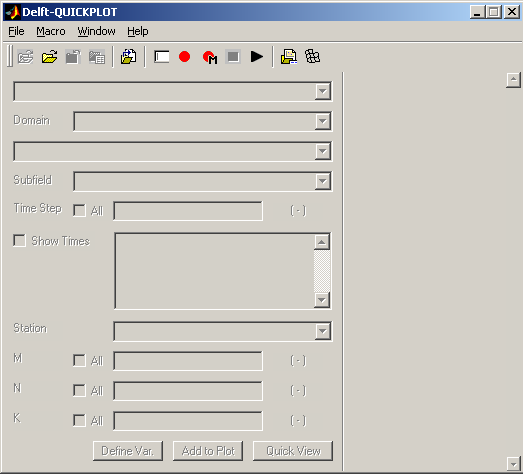
\includegraphics{Ch02/2-1.png}}
\caption{\QUICKPLOT\ main window}
\label{fig:2.1}
\end{figure}

\section{Selecting a data file}
The first step in creating a plot is opening a data file.
This can be accomplished by clicking on the Open a data file toolbar button or by selecting Open File from the File menu.
As of version 2.72, it is also possible to open a file by dragging it onto the main \QUICKPLOT\ window.

\begin{figure}
\center{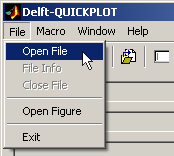
\includegraphics{Ch02/2-2a.png}
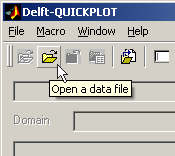
\includegraphics{Ch02/2-2b.png}}
\caption{The `File Open' command can be selected in two ways: from the \menu{File} menu and from the toolbar}
\label{fig:2.2}
\end{figure}

From the standard file selection window that appears select the data file you want to process.
The selection window contains a number of pre-configured filename filters, such as Delft3D output files \file{$\ast$.dat} or NetCDF files \file{$\ast$.nc}.
Which filters \QUICKPLOT\ shows can be adjusted via the Preferences (see \Sref{Sec:Preferences}).

\begin{Remark}
\item If the file is located on a server that supports OPeNDAP, you may also select the appropriate website using the \menu{Open URL...} menu option.
Specify for example:

\command{http://iridl.ldeo.columbia.edu/SOURCES/.WORLDBATH432/.bath/dods}

\item Although the selection interface lists for the Delft3D output files only the data files \file{$\ast$.dat}, the accompanying definition files \file{$\ast$.def} are always required for reading the data files.
Similarly, \DWAQ\ aggregated grid files consist of pairs of grid \file{$\ast$.cco} and aggregation \file{$\ast$.lga} files.
Furthermore, shape files require in general shape description \file{$\ast$.shp}, index \file{$\ast$.shx} and attribute date \file{$\ast$.dbf} files.
So, in general one has to realise that the file you select in \QUICKPLOT\ may not be the only file needed to read the data contained in it.
Have a look at \Apref{Chp:SupportedFileFormats} for an overview of the files associated with all supported file types.
\item The filename filter does not influence the automatic recognition procedure that follows the selection procedure, so any file may be selected with any filename filter active.
\item Once you have opened one or more files, the File menu contains a list of the most recently opened files (upto 9) for quick access (see \Fref{fig:2.3}).
This list is persistent between \QUICKPLOT\ sessions.
\end{Remark}

\begin{figure}
\center{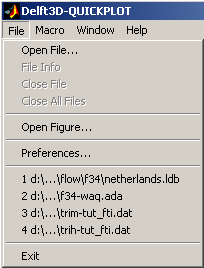
\includegraphics{Ch02/menu_file_recently_opened.png}}
\caption{The File menu contains a list of the most recently opened files}
\label{fig:2.3}
\end{figure}

After opening a \DFLOW\ map-file, the \QUICKPLOT\ interface will activate a larger part of its interface.
It will look as shown in \Fref{fig:2.5}.
The filename is indicated as the active file in the dropdown list just below the Open a data file button.
Below the filename, the data fields available from the selected file are shown.
The \button{Quick View} button for plotting the result is activated, and some plotting and export options are available from the right part of the window.
This basically indicates that you can already create your first plot now, but let us first inspect the other parts of the interface.

\begin{figure}
\center{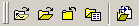
\includegraphics{Ch02/2-3.png}}
\caption{The leftmost buttons on the toolbar of the main window are used for file operations.}
\label{fig:2.4}
\end{figure}

The toolbar buttons shown above have the following meaning:

\begin{itemize}
\item The button to the left of the \button{Open a data file} button is the \button{File reload} button.
If the opened file has been changed, you can press this button to update the information initially read from the data file (e.g. number of time steps stored in the file).
This has the basically same result as re-opening the file.
However, file option settings (see below) are persistent when reloading, but they are reset upon re-opening the file.
\item Pressing the \button{Close file} button to the right of the \button{Open a data file} button removes the active file (i.e. the file selected in the dropdown list of opened files below) from the list of open files.
\item Pressing the \button{File options} button to the right of the \button{Close file} button opens another window containing some extra commands available for the selected file.
For instance, in case of a Delft3D grid file there will be buttons for opening spatial input files defined on the grid (such as bathymetry, restart files, and thin dams).
The file options dialog is an extension to the main window, i.e. all changes made in the file options dialog will immediately affect the main window and vice versa.
If you leave it open; it will update automatically if you switch between files in the main program window.
Check out the relevant section in \Apref{Sec:DefVariables} to see what functionality the file options dialog provides for your file format.
\item Finally, the last button on the right after the separator can be used to open a previously saved figure (stored MATLAB format).
\end{itemize}

The purpose of the other toolbar buttons further to the right is explained in Chapter \ref{Chp:DiggingDeeper}.

\begin{figure}
\center{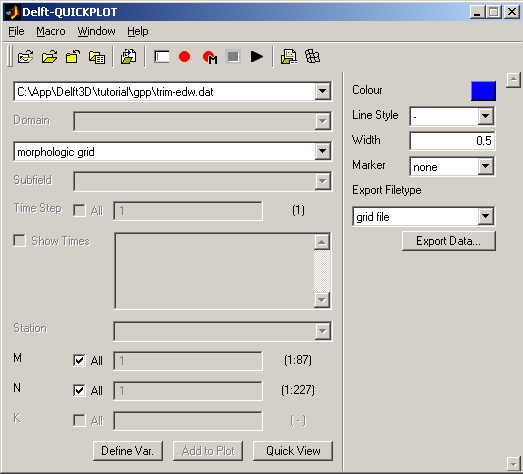
\includegraphics{Ch02/2-4.png}}
\caption{User interface after opening a \DFLOW\ map file.}
\label{fig:2.5}
\end{figure}

\section{Selecting a data field}
The next step in creating a plot is selecting the quantity or data field from the file to be plotted.
The data fields available from the active file are shown in a dropdown list below the name of the file.
Click on the selected field (in the example: `morphologic grid') to expand the list and to select another data field as shown in \Fref{fig:2.6}.
The supported file formats and the data fields that may be contained in them are listed in \Apref{Chp:SupportedFileFormats}.

\begin{figure}
\center{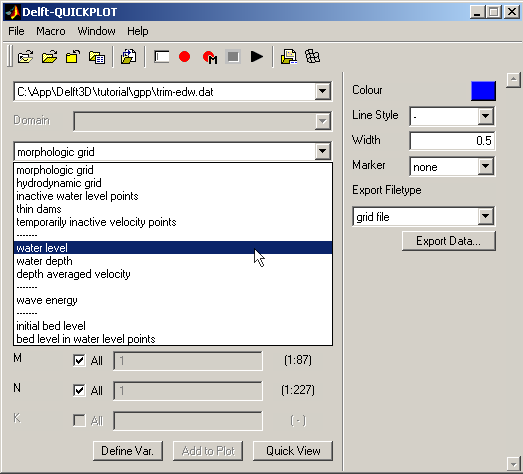
\includegraphics{Ch02/2-5.png}}
\caption{List of data fields in the \DFLOW\ map file.}
\label{fig:2.6}
\end{figure}

Different quantities allow for different types of plots and, therefore, the lists of plot and export options in the right part of the window will adapt to your selection.
\Fref{fig:2.7} shows the list of options if the water level (or any other scalar 2D quantity) is selected; the options will be discussed in Chapter \ref{Chp:PlottingOptions}.
Furthermore, the number of time steps depends on the selected data field; the example file contains 6 time steps for the water level as indicated by the edit box below the datafield list box.

The domain selection box between the file selection box and the datafield selection box is only active when the file may contain multiple domains.
Similarly, the subfield selection box immediately below the datafield selection box is only active when the datafield contains multiple subfields (e.g. the datafield `sediment transport' may have subfields for sediment fractions 1, 2, etc.)

\begin{figure}
\center{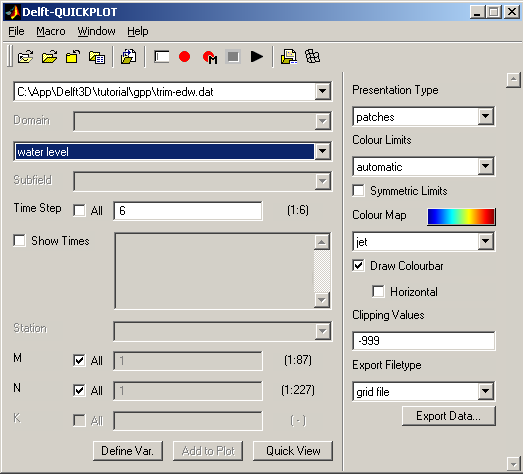
\includegraphics{Ch02/2-6.png}}
\caption{The list of plot options is changed after selection of the water level from the dropdown list.}
\label{fig:2.7}
\end{figure}

\section{Selecting a time}
When the selected data field is time-dependent, you must select which time step you want to plot.
The default setting is to plot the last time step for 1D, 2D and 3D quantities and all time steps for scalar quantities.
In the case of \Fref{fig:2.7} time step 6 has been selected.

\begin{Remark}
\item The valid range of time step numbers is indicated to the right of the time step edit box.
\item If you want to see the times associated with the time steps stored in the file, check the Show Times checkbox (see \Fref{fig:2.8}).
Reading and displaying a large number of times can be very time consuming and you should be careful when opening data files (generally history files) containing a large number of time steps: uncheck the Show Times checkbox first.
\item The Show Times checkbox is automatically disabled if the number of time steps is larger than 30,000.
\item Multiple time steps can be selected by typing the time steps in the Time Step edit box.
This is particularly useful if the data file contains many time steps; type for instance 1:10:301 if you want to plot every 10th time step of a series of 301 time steps.
\item The extraction of a time-series from a map-file is typically carried out by reading for each selected time step the whole domain and selecting only the requested point.
This procedure is more flexible yet also slower than plotting time-series from a dedicated history file.
\end{Remark}

\begin{figure}
\center{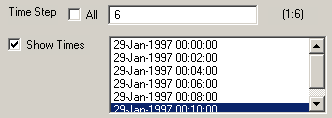
\includegraphics{Ch02/2-7.png}}
\caption{Optional listing of the times associated with the various time steps.}
\label{fig:2.8}
\end{figure}

\section{Selecting a location}
The next step is to select the location for which to plot.
The default setting is to plot the whole domain for 1D, 2D and 3D quantities.
In the case of \Fref{fig:2.7} this is reflected by the fact that all M and N indices have been selected.
If instead of a 2D plot of the whole domain, you want a plot of a cross-section along an M grid line uncheck the All checkbox associated with M and specify the M-value of the desired grid line as shown in \Fref{fig:2.9}.

\begin{figure}
\center{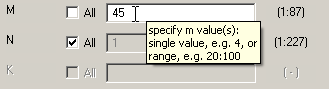
\includegraphics{Ch02/2-8.png}}
\caption{Selection of a cross-section along a grid line in M direction: one M value, all N values.}
\label{fig:2.9}
\end{figure}

\begin{Remark}
\item The valid range of grid indices is indicated to the right of the M, N and K edit boxes, respectively.
Depending on the origin of the data, the indicated range of grid points may include an additional row of points added due to staggering of the variables on the computational grid.
As a consequence, the first and last grid lines may or may not have data defined on it.
\item Instead of selecting a block of M and N indices, you may want to select a generic cross-section that runs piecewise along grid lines (or diagonal lines).
This can be accomplished by selecting the (MN) option as shown in \Fref{fig:2.10}.
The M and N pairs should be separated using spaces, commas or semi-colons.
Once the input has been parsed \QUICKPLOT\ will separate to co-ordinate pairs by semi-colons and the co-ordinate indices by commas as shown in the figure.
See also \Sref{Sec:GridView} on selecting such cross-sections interactively.
\item The aforementioned text describes the situation for a structured mesh.
For network or unstructured mesh, you may have only one spatial M index rather than two M and N indices.
All functions will still be available, but selecting a slice or subdomain is typically not as easy as selecting a simple range of M indices.
For these case, the use of the Grid View window is strongly recommended (see \Sref{Sec:GridView}).
\item Another option is to select an arbitrary cross-section using (x,y) co-ordinates.
This feature is activated using the (XY) option as shown in \Fref{fig:2.11}.
The x and y co-ordinates should be separated using spaces, commas or semi-colons.
Once the input has been parsed \QUICKPLOT\ will separate to co-ordinate pairs by semi-colons and the co-ordinate indices by commas as shown in the figure.
See also \Sref{Sec:GridView} on selecting such cross-sections interactively.
\item It is currently not yet possible to make generic horizontal slices (such as along Z-planes instead of K-planes).
\end{Remark}

\begin{figure}
\center{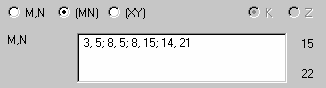
\includegraphics{Ch02/piece_wise_along_grid_lines.png}}
\caption{Selection of a cross-section piecewise along a grid lines.}
\label{fig:2.10}
\end{figure}

\begin{figure}
\center{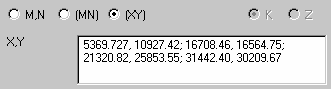
\includegraphics{Ch02/arbitrary_cross_section_using_xy.png}}
\caption{Selection of an arbitrary cross-section using (x,y) co-ordinates.}
\label{fig:2.11}
\end{figure}

If you want a time-series plot at any computational point of the grid from a map file, select All (or multiple) time steps and (as appropriate) one M, one N and one K index.
If you have opened a history file, for instance a \DFLOW\ trih-file, the spatial dimensions M and N will not be available.
Instead you can select the observation point or cross-section name from the station list as shown in \Fref{fig:2.12}.
By default the stations are listed in the same order as they are available in the data file; typically, this matches the order of the stations in the input files.
As of version 2.72, it is possible to modify the order of the stations by selecting a sorting option via Preferences, see \autoref{Sec:Preferences}.

\begin{figure}
\center{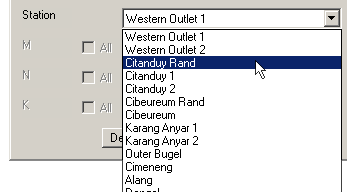
\includegraphics{Ch02/2-9.png}}
\caption{Example of the station list in case of a history file.}
\label{fig:2.12}
\end{figure}

\section{Creating a plot}
You can now plot the data by pressing the Quick View button.
Depending on the data field selected, the selected time step and the selected spatial extent, you will get a 2D plot, a cross-sectional plot or a time-series plot.
\Fref{fig:2.13} until \Fref{fig:2.15} show some results.

\begin{Remark}
\item If you have selected multiple time steps and a spatially extended plot domain (i.e., all or multiple M, N or K co-ordinates), the Quick View button will have changed into a Quick Animate button.
Pressing the button will cause the program to animate the selected plot by looping over the selected time steps.
The same result can also be obtained by selecting one time step initially and using the Animation menu in the plot.
\item It is currently not possible to plot data sets on a 3D domain (i.e. all or multiple M, N and K co-ordinates selected).
Always specify a single M, N or K co-ordinate for 3D data sets.
\end{Remark}

If there are multiple time steps and if you have selected only one, or if you have selected only one M, N or K co-ordinate, the plot will contain an active slider in the lower left corner of the plot.
You can select other time steps and other spatial co-ordinates using that slider.
See Chapter \ref{Sec:DefVariables} for information on how to use the slider, how to create animations, how to combine plots, and how to define your own variables.
For more information on the various plot styles supported by \QUICKPLOT\ see \Sref{Chp:PlotStyles}.
For plot options see \Sref{Chp:PlottingOptions}, and for more advanced plotting options see \Sref{Chp:DiggingDeeper}.

\begin{figure}
\center{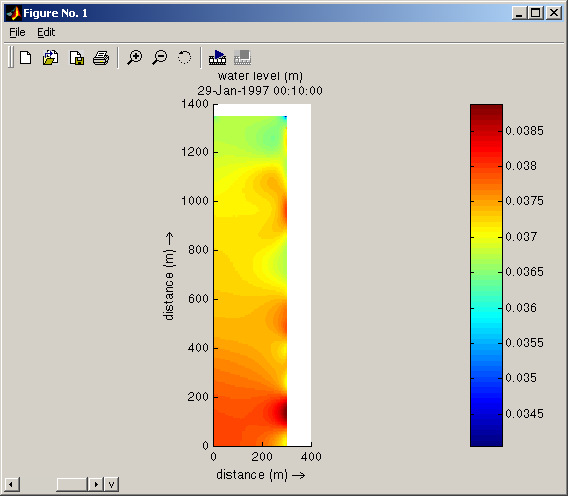
\includegraphics[width=125mm]{Ch02/2-10.png}}
\caption{2D Plot of the water levels.}
\label{fig:2.13}
\end{figure}

\begin{figure}
\center{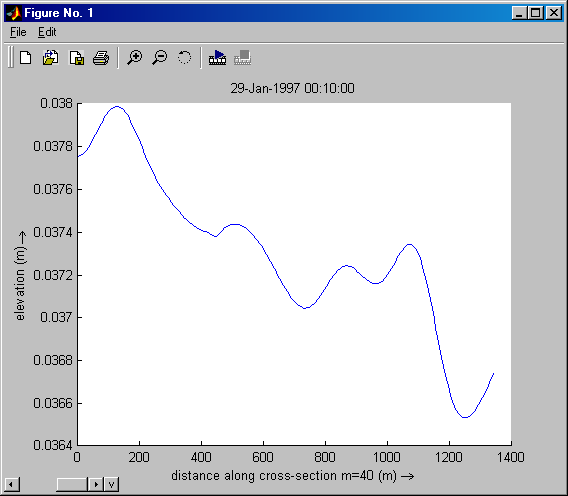
\includegraphics[width=125mm]{Ch02/2-11.png}}
\caption{Plot of the water levels along a grid line of constant M.}
\label{fig:2.14}
\end{figure}

\begin{figure}
\center{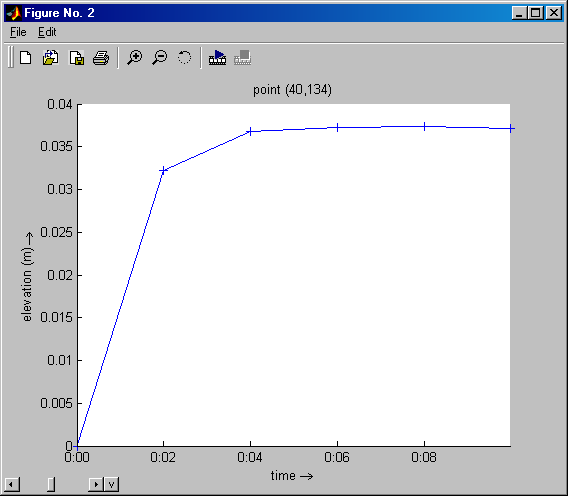
\includegraphics[width=125mm]{Ch02/2-12.png}}
\caption{Time-series plot of the convergence of the water levels at point M=40, N=134 to a stationary solution.
Markers added for clarity (see \Sref{Sec:Markers})..}
\label{fig:2.15}
\end{figure}
